\documentclass[14pt]{beamer}
\usepackage[T2A]{fontenc}
\usepackage[utf8]{inputenc}
\usepackage[english,russian]{babel}
\usepackage{amssymb,amsfonts,amsmath,mathtext}
\usepackage{cite,enumerate,float,indentfirst}

\graphicspath{{images/}}

\usetheme{Pittsburgh}
\usecolortheme{whale}

\setbeamercolor{footline}{fg=blue}
\setbeamertemplate{footline}{
  \leavevmode%
  \hbox{%
  \begin{beamercolorbox}[wd=.333333\paperwidth,ht=2.25ex,dp=1ex,center]{}%
    А.В.~Сидорин, МГТУ им. Баумана
  \end{beamercolorbox}%
  \begin{beamercolorbox}[wd=.333333\paperwidth,ht=2.25ex,dp=1ex,center]{}%
    Москва, 2015
  \end{beamercolorbox}%
  \begin{beamercolorbox}[wd=.333333\paperwidth,ht=2.25ex,dp=1ex,right]{}%
  Стр. \insertframenumber{} из \inserttotalframenumber \hspace*{2ex}
  \end{beamercolorbox}}%
  \vskip0pt%
}

\newcommand{\itemi}{\item[\checkmark]}

\title{\small{Новая модификация метода анализа кодов программ на основе резюме для тестирования сложных программных комплексов}}
\author{\small{%
\emph{Выступающий:}~А.В.~Сидорин\\%
\emph{Руководитель:}~доцент,~к.ф.-м.н.~Т.Н.~Романова}\\%
\vspace{30pt}%
Московский государственный технический университет имени Н. Э. Баумана%
\vspace{20pt}%
}
\date{\small{Москва, 2015}}

\begin{document}

\maketitle

\begin{frame}
\frametitle{Цель работы}
\begin{itemize}
  \item Построение метода анализа крупных программных комплексов, разработанных с использованием языков C и C++, способного осуществлять анализ проектов масштаба ОС Android и ОС Tizen (порядка 5--20~млн. строк кода) за приемлемое время и обеспечивающего достаточное покрытие путей выполнения программы.
\end{itemize}
\end{frame}

\begin{frame}
\frametitle{Актуальные проблемы статического анализа}
\begin{itemize}
  \item Необходимость поиска компромисса между качеством, полнотой и временем анализа
  \item Экспоненциальная сложность наиболее точных и полных видов статического анализа делает их ограниченно применимыми для анализа крупных программных систем
  \item Проблема улучшения производительности методов статического анализа является актуальной   
\end{itemize}
\end{frame}

\begin{frame}[allowframebreaks]
\frametitle{Поставленные задачи}
\begin{enumerate}
  \item Разработать метод межпроцедурного анализа программ, пригодный для анализа крупных программных проектов, а также расширяемый на различные виды проверок
  \item Разработать метод межмодульного анализа программ, разработанных с использованием языков C и C++
  \item Разработать метод отображения результатов анализа при использовании предложенного метода межпроцедурного анализа
  \item Для экспериментального подтверждения эффективности предложенных методов реализовать их и осуществить тестирование разработанных методов на реальных программных проектах
  \item По результатам тестирования сделать выводы о пригодности разработанного метода, о его применимости для анализа крупных программных комплексов и качестве анализа кода программ
\end{enumerate}
\end{frame}

\begin{frame}[allowframebreaks]
\frametitle{Основные положения, выносимые на защиту}
\begin{enumerate}
  \item Новая модификация метода межпроцедурного анализа программ на основе резюме для метода символьного выполнения для программ, разработанных с использованием языков C и C++
  \item Метод межмодульного анализа программ, разработанных с использованием языков C и C++, архитектура анализатора, эвристики, связанные с объединением синтаксических деревьев различных единиц трансляции
  \item Метод построения отчёта о дефекте при использовании метода резюме для метода символьного выполнения
\end{enumerate}
\end{frame}

\begin{frame}[allowframebreaks]
\frametitle{Мотивация}
\begin{itemize}
  \item Необходимость автоматизации поиска дефектов в крупных и критичных по качеству программных продуктах требует выполнения анализа с высокой полнотой и точностью
  \item При использовании метода символьного выполнения можно достичь указанных характеристик
  \begin{itemize}
    \item Анализ, чувствительный к пути выполнения и потоку управления
  \end{itemize}

  \item Для данного метода существует проблема экспоненциального роста количества путей при увеличении размера программы
  \item Межпроцедурный анализ усугубляет данную проблему, увеличивая количество возможных путей выполнения при использовании контекстно-чувствительного анализа
  \item Задача разработки метода МПА, в меньшей степени затронутого данной проблемой, является актуальной.
\end{itemize}
\end{frame}

\begin{frame}[allowframebreaks]
\frametitle{Мотивация~--- языки программирования C и C++}
\begin{itemize}
  \item Большое количеством видов потенциальных ошибок, которые может допустить программист
  \begin{itemize}
    \item Неправильная работа с~указателями
    \item Неопределённое или зависящее от реализации поведение
  \end{itemize}
  \item Наиболее распространённые и~известные языки
    \begin{itemize}
    \item Большое количество существующего системного и~прикладного ПО
    \item ПО с высокими требованиями к производительности
    \item Низкоуровневые компоненты, такие как компоненты операционных систем и~драйверы
  \end{itemize}
  \item Проблема глубокого анализа программ на языках C и C++ является актуальной.
\end{itemize}
\end{frame}

\begin{frame}[allowframebreaks]
\frametitle{Предлагаемая модификация метода резюме}
\begin{itemize}
  \item Анализ функции вне контекста вызова с последующим уточнением контекста
  \item Позволяет не анализировать одну и ту же функцию многократно, а использовать её резюме
  \item Использовался различными исследователями для реализации обособленных видов проверок
\end{itemize}
\end{frame}

\begin{frame}[allowframebreaks]
\frametitle{Предлагаемая модификация метода резюме}
\begin{itemize}
  \item Цель исследования: построение многоцелевого анализатора для языков C и C++
  \item Решённые проблемы:
  \begin{itemize}
    \item Поддержка модели памяти C/C++, включая арифметику указателей, наследования и выравнивания полей структур
    \item Отсечение недостижимых путей выполнения
    \item Поддержка сложных алгоритмов поиска дефектов и их одновременного использования при МПА методом резюме
  \end{itemize}
\end{itemize}
\end{frame}

\begin{frame}
\frametitle{Структура резюме}
\begin{itemize}
  \item В предлагаемой модификации, \textit{резюме} представляет собой набор \textit{ветвей резюме}, каждая из которых соответствует листу графа выполнения функции
  \item Соответственно, каждая ветвь задаёт класс эквивалентности относительно параметров функции
  \item Каждая ветвь содержит предусловия, при которых достижима данная ветвь, и постусловие, которое является эффектом ветви выполнения функции на состояние программы.
\end{itemize}
\end{frame}

\begin{frame}
\frametitle{Поддержка модели памяти в резюме}
\begin{itemize}
  \item Для анализа функции в контексте вызова производится \textit{актуализация} символьных значений
  \begin{enumerate}
    \item Вне контекста строится цепочка доступа вида \\ \textit{<<параметр функции 1 $\rightarrow$ поле lock $\rightarrow$ элемент 2>>}
    \item В контексте вызова цепочка доступа применяется к региону памяти, являющемуся фактическим аргументом при вызове функции
  \end{enumerate}
\end{itemize}
\end{frame}

\begin{frame}[allowframebreaks]
\frametitle{Применение резюме. Отсечение недостижимых путей}
\begin{itemize}
  \item Каждое символьное значение имеет своё множество возможных конкретных значений
  \item Пересечение этих диапазонов для фактических и формальных параметров становится новым диапазоном конкретных значений фактического параметра в вызывающей функции
  \item Пустое пересечение означает недостижимость данной ветви выполнения
  \item Если ветвь выполнения достижима, применяются постусловия, включающие в себя привязку новых символьных значений к регионам памяти, в которые произошла запись в вызываемой функции
  \item Символьное значение, возвращаемое функцией, также подвергается актуализации и становится значением выражения-вызова функции.
\end{itemize}
\end{frame}

\begin{frame}[allowframebreaks]
\frametitle{Проверки при применении резюме}
\begin{itemize}
  \item Каждый проверяющий модуль имеет своё состояние (type state)
  \item Каждый проверяющий модуль может создавать своё резюме и применять его независимо как от других модулей, так и от остальных компонентов анализатора, что позволяет реализовывать МПА методом резюме для проверок произвольного вида
  \item В резюме проверяющего модуля обычно входят изменения состояния программы и отложенные проверки
  \item В рамках данной работы МПА методом резюме был реализован для проверяющих модулей различного назначения:
    \begin{itemize}
    \item Строковое переполнение
    \item Корректность операций над файловыми дескрипторами
    \item Проверка корректности синхронизации в многопоточной среде
    \item Целочисленное переполнение
    \item Запись в переменную константного типа
  \end{itemize}
\end{itemize}
\end{frame}

\begin{frame}[allowframebreaks]
\frametitle{О полноте анализа при использовании различных методов МПА}
\textbf{Теорема 1}. Если при использовании проверки с помощью метода встраивания результатом проверки является предупреждение, выданное в некотором узле графа выполнения программы, то при использовании метода резюме для той же функции верхнего уровня и того же набора вызываемых функций результатом проверки методом резюме также является предупреждение, выданное в узле графа выполнения вызывающей функции или в одном из узлов графов выполнения вызываемых функций.

\textbf{Теорема 2}. При использовании отложенной проверки в конце анализа функции верхнего уровня при использовании МПА методом встраивания и МПА методом резюме множества срабатываний совпадают.
\end{frame}

\begin{frame}
\frametitle{Построение отчёта}
\begin{itemize}
  \item Отчёт должен содержать полную информацию о пути выполнения, на котором наблюдается дефект
  \item При использовании метода резюме происходит потеря информации о пути выполнения внутри вызываемой функции
  \item Для решения этой проблемы предлагается использовать хранение ссылки на узел графа вызываемой функции, соответствующий ветви применения резюме.
\end{itemize}
\end{frame}

\begin{frame}
\frametitle{Построение отчёта~--- пример 1}
\begin{figure}[H]
  \center{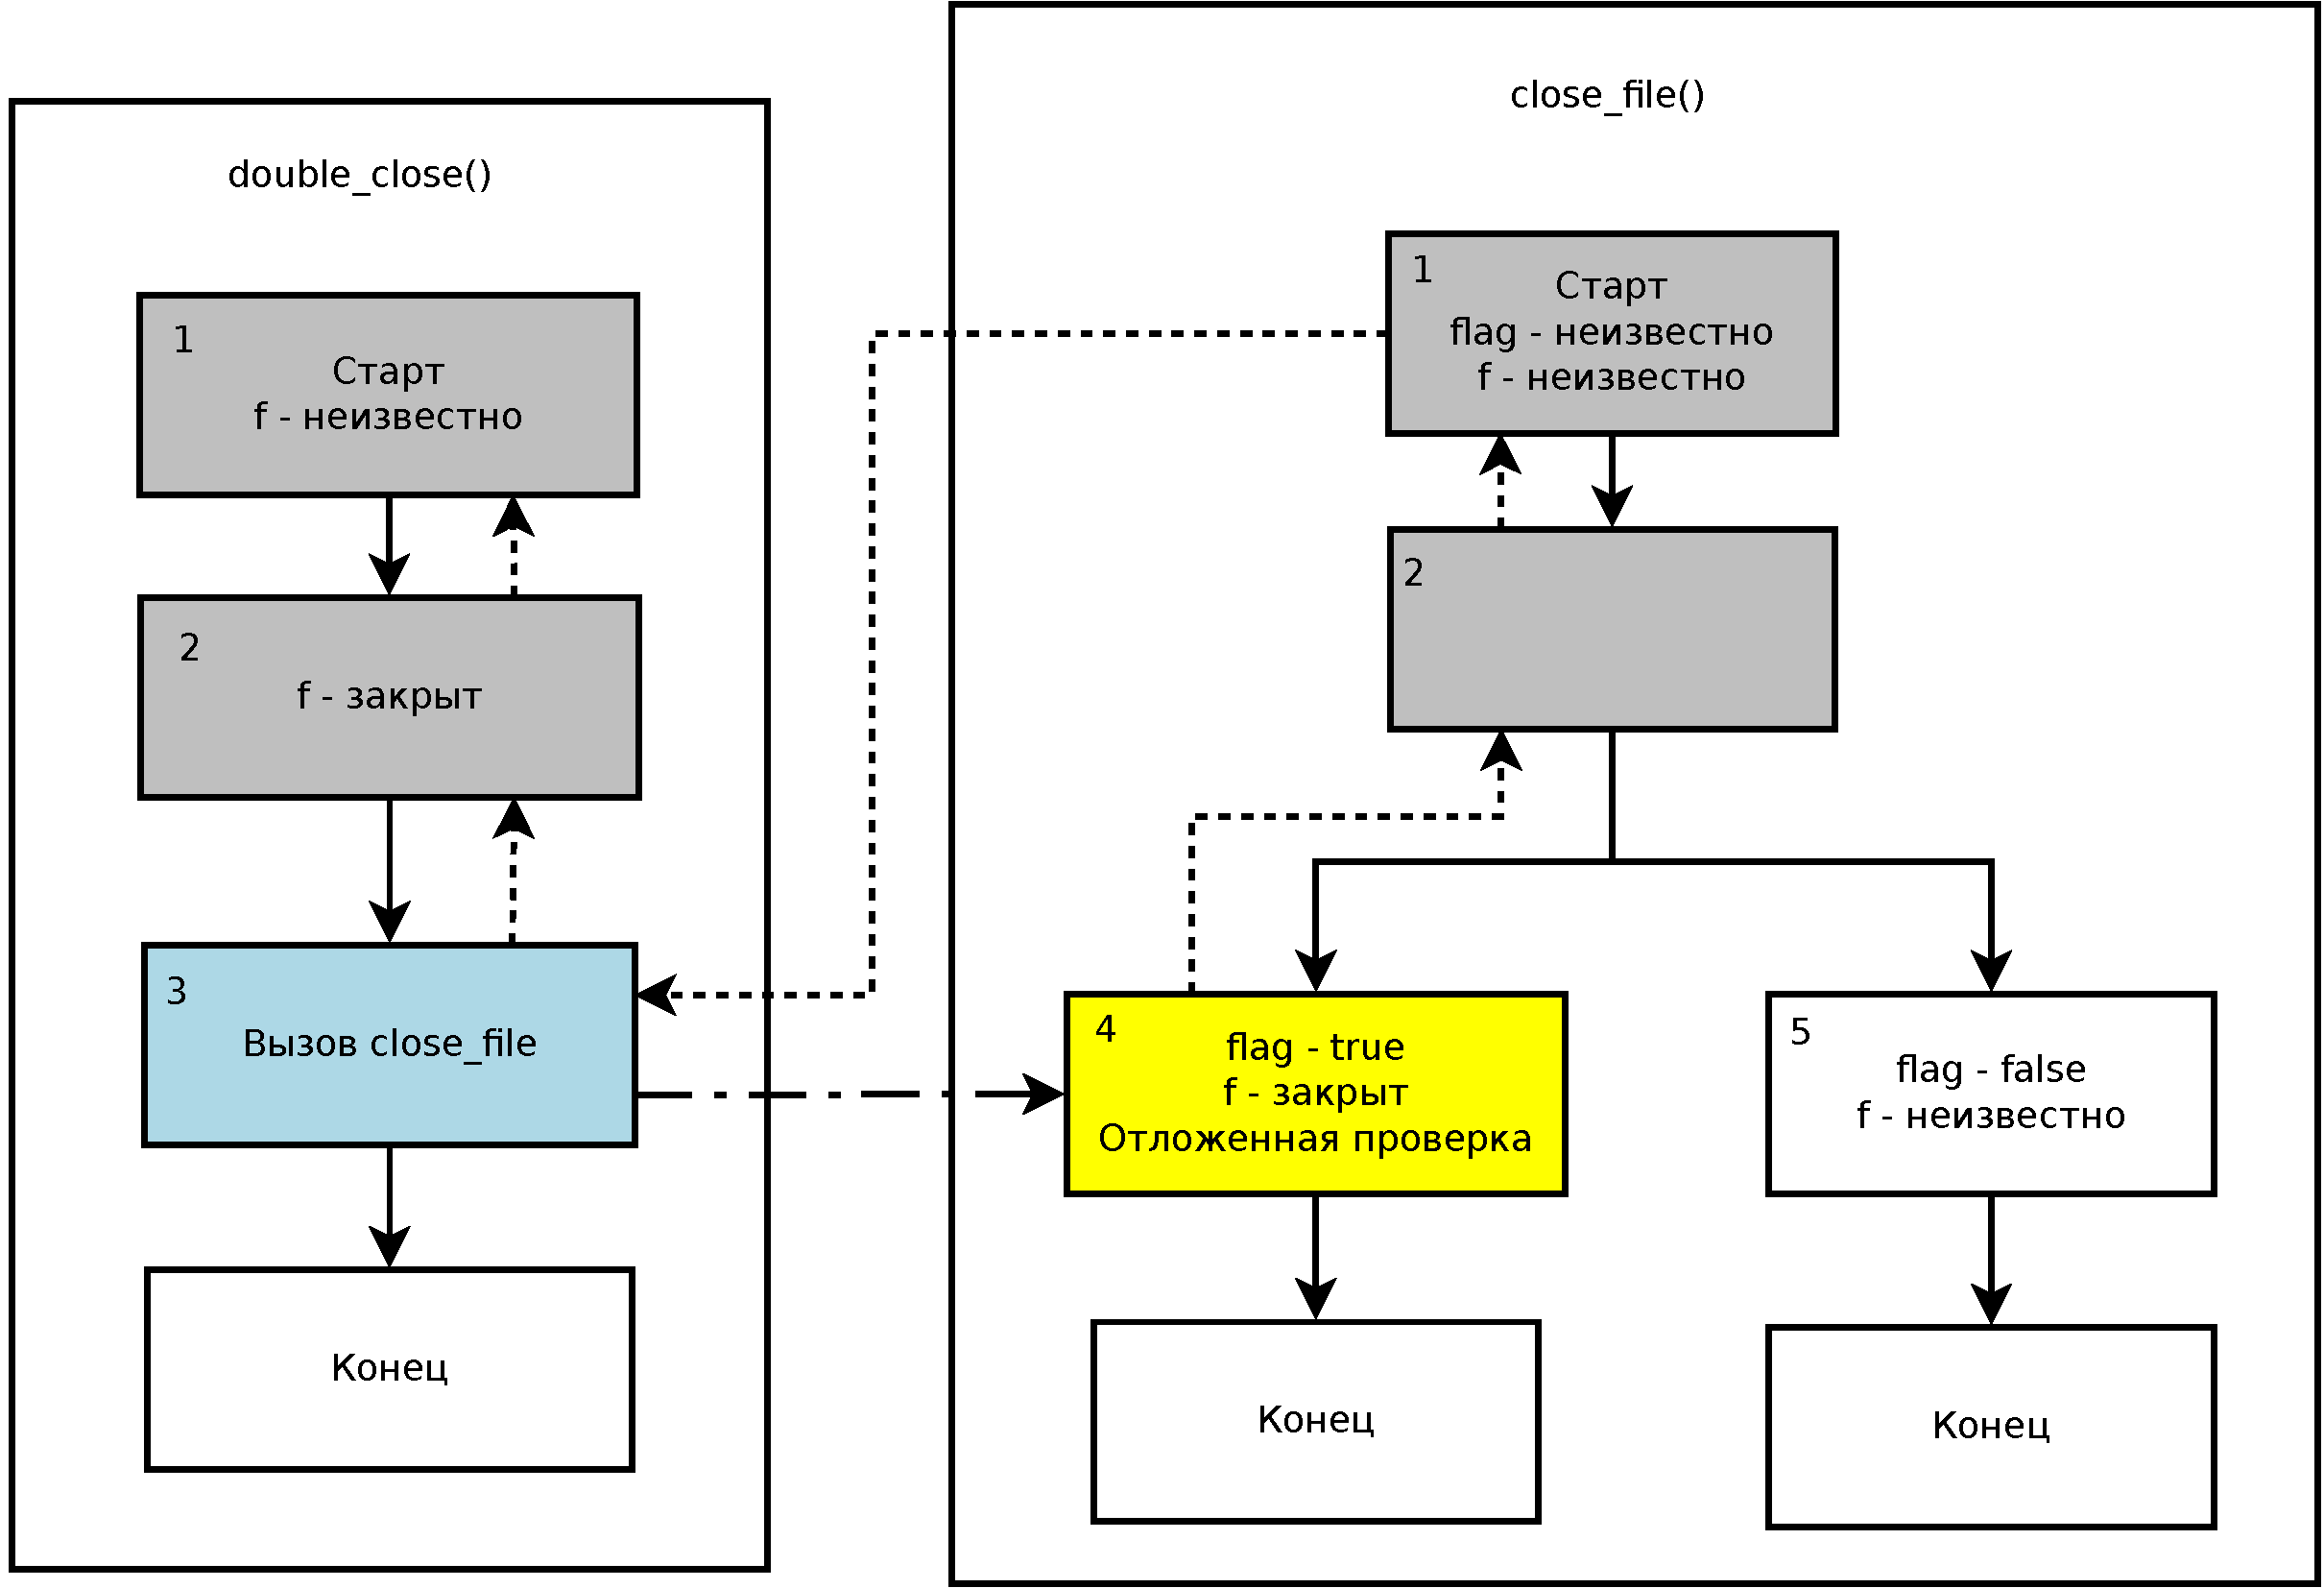
\includegraphics[width=1\linewidth]{../Dissertation/images/call-trace.pdf}}
\end{figure}
\end{frame}

\begin{frame}
\frametitle{Построение отчёта~--- пример 2}
\begin{figure}[h]
  \center{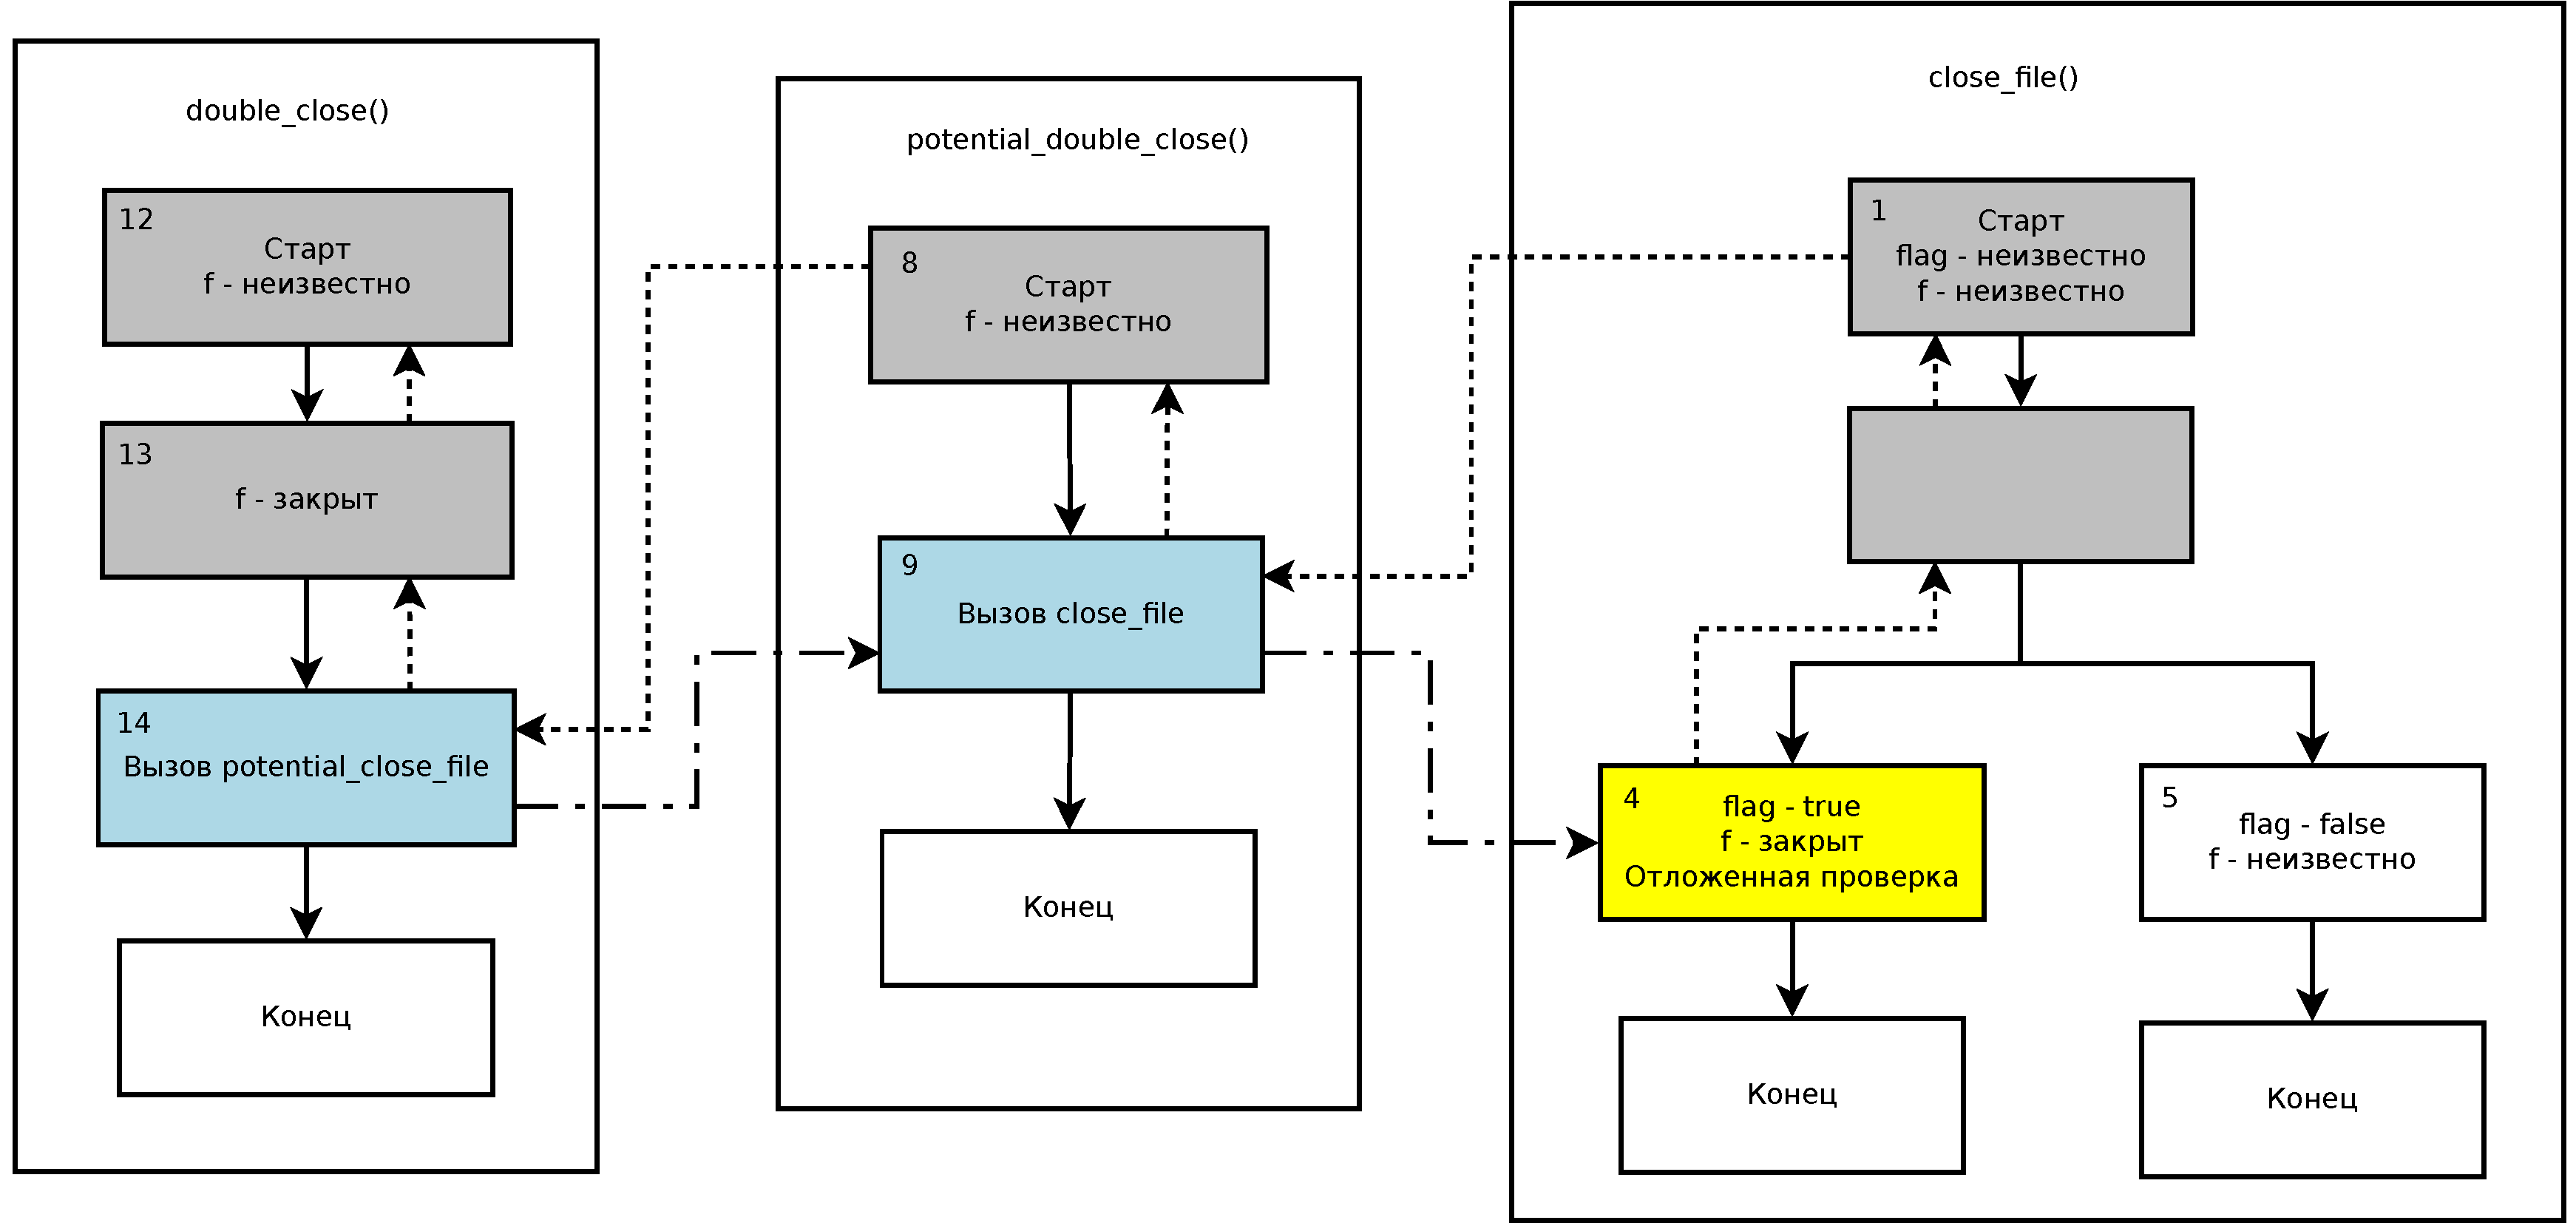
\includegraphics[width=1\linewidth]{../Dissertation/images/call-trace-multiple.pdf}}
\end{figure}
\end{frame}

\begin{frame}
\frametitle{Межмодульный анализ}
\begin{itemize}
  \item C и C++~--- языки с поддержкой раздельной компиляции
  \item Для анализа крупных программ необходимо обрабатывать функции, определённые в различных единицах трансляции
  \item Для решения этой проблемы предлагается использовать слияние синтаксических деревьев единиц трансляции.
    \begin{itemize}
      \item Данный метод позволяет сохранять всю доступную информацию о программе без потери при преобразованиях
    \end{itemize}
\end{itemize}
\end{frame}

\begin{frame}
\frametitle{Межмодульный анализ~--- реализация}
В данной работе реализован межмодульный анализ, состоящий из трёх фаз
\begin{enumerate}
  \item На первой фазе происходит перехват команд построения проекта
  \begin{enumerate}
    \item Построение синтаксических деревьев единиц трансляции с сохранением их на носитель
    \item Сохранение данных о требуемых и имеющихся определениях функций
  \end{enumerate}
  \item На второй фазе строится соответствие между требуемыми и имеющимися функциями, производится топологическая сортировка графа вызовов
  \item На третьей фазе происходит запуск анализа со слиянием синтаксических деревьев.
\end{enumerate}
\end{frame}

\begin{frame}[allowframebreaks]
\frametitle{Межмодульный анализ~--- решаемые проблемы}
\begin{enumerate}
  \item Необходимость различения синтаксических деревьев и функций различных архитектур, а также перегруженных функций
    \begin{itemize}
      \item Для поиска используются сигнатуры, содержащие соответствующую информацию
    \end{itemize}
  \item Длительный рекурсивный поиск
  \begin{enumerate}
    \item Объявления с различными именами являются различными
    \item Объявления различных разновидностей являются различными
    \item Объявления из одного файла с одинаковыми текстовыми позициями начала и завершения считаются совпадающими
  \end{enumerate}
  \item Сложные зависимости между импортируемыми объявлениями при рекурсивном импорте
    \begin{itemize}
      \item Необходимо переупорядочивать сливаемые объявления
    \end{itemize}
\end{enumerate}
\end{frame}


\begin{frame}
\frametitle{Покрытие~--- внутримодульный анализ}
\begin{figure}[h]
  \center{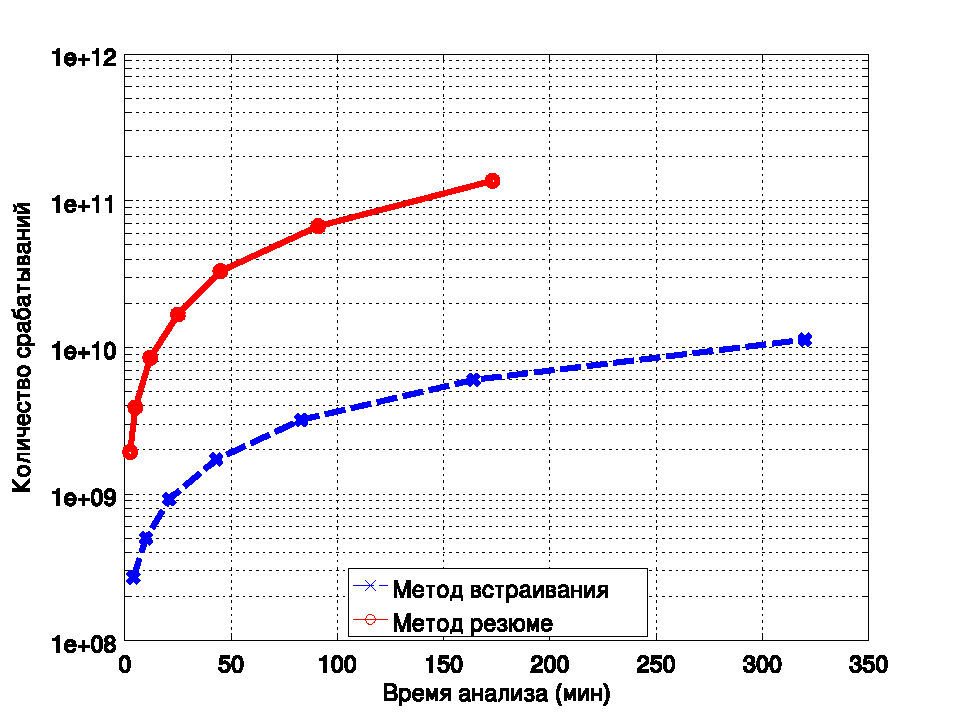
\includegraphics[width=0.8\linewidth]{../Dissertation/images/single-nodes.pdf}}
\end{figure}
\end{frame}

\begin{frame}
\frametitle{Покрытие~--- межмодульный анализ}
\begin{figure}[h]
  \center{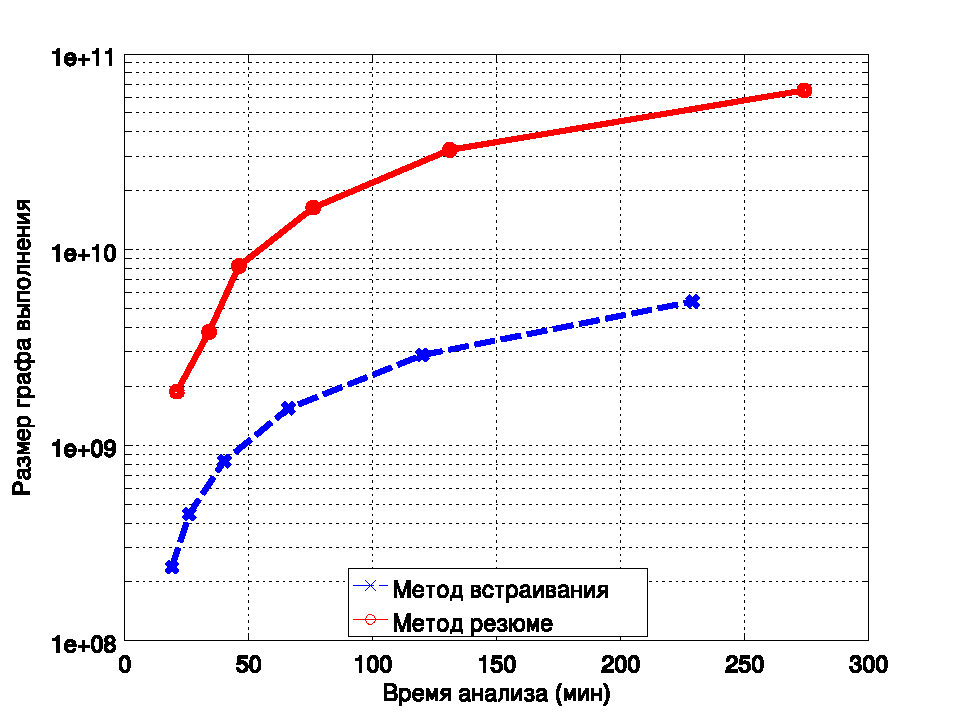
\includegraphics[width=0.8\linewidth]{../Dissertation/images/xtu-nodes.pdf}}
\end{figure}
\end{frame}

\begin{frame}
\frametitle{Поиск дефектов~--- внутримодульный анализ}
\begin{figure}[h]
  \center{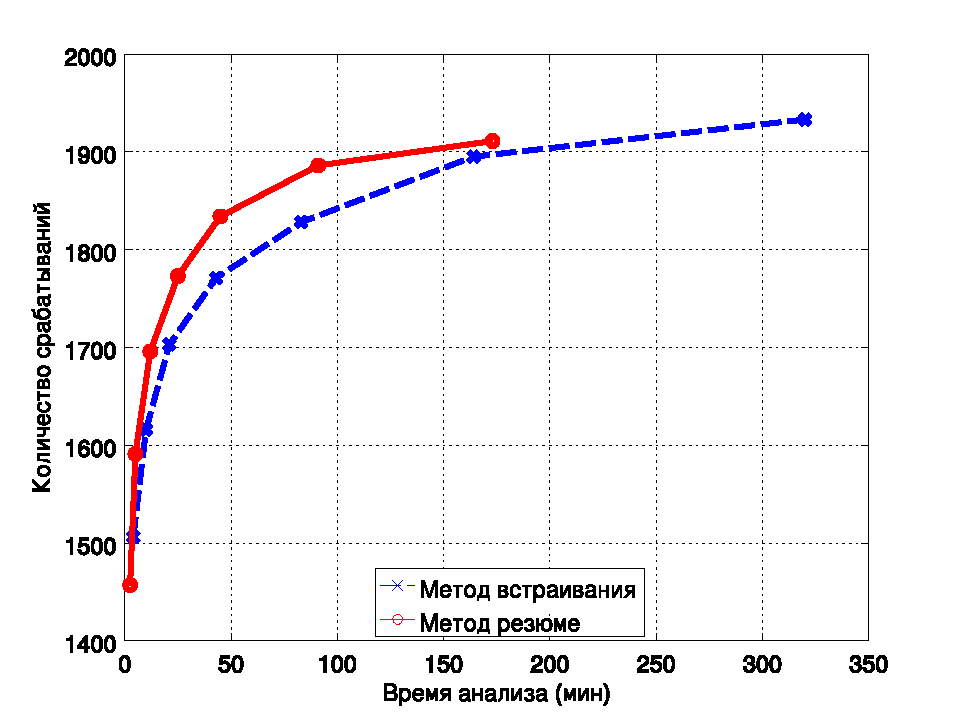
\includegraphics[width=0.8\linewidth]{../Dissertation/images/single-unique.pdf}}
\end{figure}
\end{frame}

\begin{frame}
\frametitle{Поиск дефектов~--- межмодульный анализ}
\begin{figure}[h]
  \center{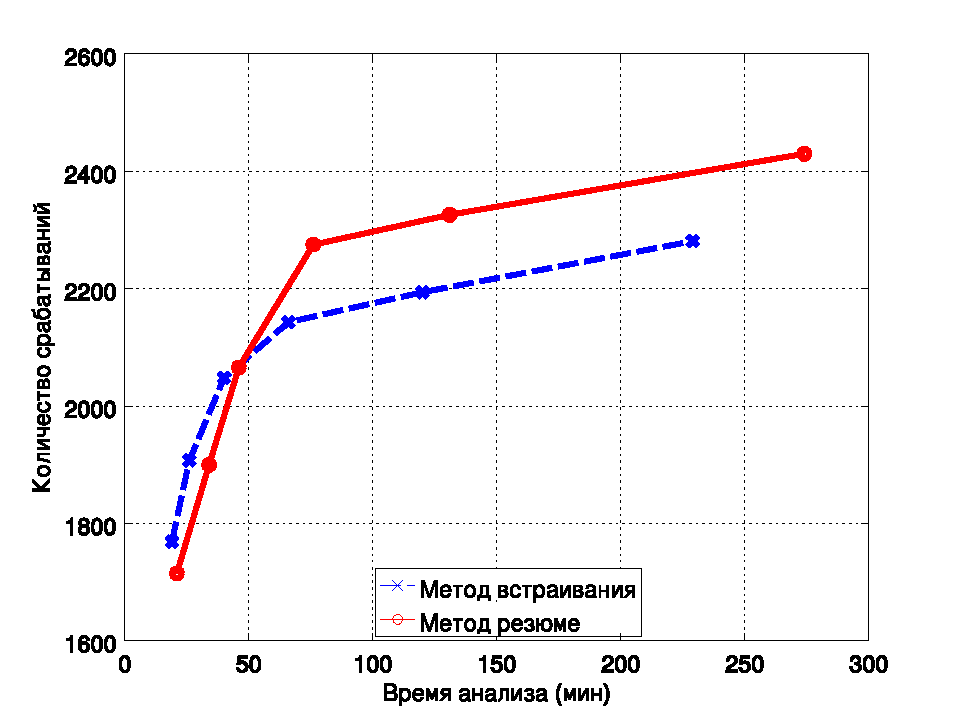
\includegraphics[width=0.8\linewidth]{../Dissertation/images/xtu-unique.pdf}}
\end{figure}
\end{frame}

\begin{frame}[allowframebreaks]
\frametitle{Выводы}
Результаты тестирования в сравнении с методом встраивания при одинаковом времени работы анализатора показали следующее:
\begin{enumerate}
  \item уйти от экспоненциального роста времени анализа полностью не удалось, хотя был продемонстрирован значительный рост производительности анализа
  \item покрытие операторов программы увеличилось на порядок (в 15--20 раз)
  \item скорости поиска дефектов также увеличилась: то же количество уникальных дефектов можно обнаружить в 2--3 раза быстрее
  \item удалось сохранить точность анализа, которая составила от 80\% до 84\% в зависимости от настроек анализатора
\end{enumerate}
\end{frame}
%%%%%%%%%%%%%%%%%%%%%%%%%%%%%%
\begin{frame}
\frametitle{Перспективы развития работы}
\begin{itemize}
  \item Исследование и реализация возможностей повторного использования резюме при межмодульном анализе
  \item Моделирование компоновщика для поиска требуемых определений функций
  \item Реализация МПА методом резюме для большего количества проверяющих модулей, включая проверки безопасности
\end{itemize}
\end{frame}

\begin{frame}[allowframebreaks]
\frametitle{Результаты работы}
\begin{itemize}
  \item Разработана новая модификация метода межпроцедурного анализа программ на основе резюме для метода символьного выполнения для программ, реализованных с использованием языков C и C++. Данный метод анализа позволяет производить анализ с высоким качеством и полнотой, однако имеет экспоненциальную сложность, связанную с проблемой роста количества путей с увеличением объёма программы (path explosion), что делает задачу улучшения его производительности особенно актуальной. Важными особенностями разработанного метода является поддержка проверок произвольного вида и их одновременного выполнения, а также поддержка модели памяти, используемой в языках C и C++, в том числе, с учётом арифметики указателей, наследования и выравнивания полей структур.
  \item Разработан метод межмодульного анализа программ, реализованных с использованием языков C и C++ для статического анализатора, использующего в качестве входных данных непосредственно исходный код программы. Использование промежуточного представления в виде синтаксического дерева программы позволяет производить анализ без потери информации о программе.
  \item Разработан метод построения отчёта о дефекте при использовании предложенной модификации метода резюме для метода символьного выполнения. Данный метод позволяет строить информативный межпроцедурный отчёт, включающий показ переходов, выполнимых условий и представляющих интерес событий в процессе выполнения программы.
  \item Для экспериментального подтверждения эффективности предложенных методов они были реализованы их для использования в приложении-анализаторе (Clang Static Analyzer, анализатор с открытым исходным кодом). Было осуществлено тестирование разработанных методов на реальных программных проектах~--- пакетах пользовательского окружения ОС Android.
  \item По результатам тестирования сделан выводы о пригодности разработанного метода. Несмотря на сохранение экспоненциальной сложности анализа, тесты показали, что скорость поиска дефектов и покрытие путей тестируемых программы увеличились, а качество анализа кода программ сохранилось на том же уровне.
\end{itemize}
\end{frame}

\begin{frame}
\begin{center}
Спасибо за внимание!
\end{center}
\end{frame}

% \begin{frame}
% \frametitle{Формулы}
% $$
% \left\{
%   \begin{array}{rl}
%     \dot x = & \sigma (y-x) \\
%     \dot y = & x (r - z) - y \\
%     \dot z = & xy - bz
%   \end{array}
% \right.
% $$
% \end{frame}
% 
% \begin{frame}
% \frametitle{Составное изображение}
% \begin{figure}[h]
%   \begin{minipage}[h]{0.49\linewidth}
%     \textbf{Составная \\ подпись 1}
%     \center{\includegraphics[width=1\linewidth]{knuth1}}
%   \end{minipage}
%   \hfill
%   \begin{minipage}[h]{0.49\linewidth}
%     \textbf{Составная \\ подпись 2}
%     \center{\includegraphics[width=1\linewidth]{knuth2}}
%   \end{minipage}
% \end{figure}
% \end{frame}
% 
% \begin{frame}
% \frametitle{Таблица}
% \begin{tabular}{|l|l|}
% \hline
% \textbf{Заголовок 1} & \textbf{Заголовок 2} \\
% \hline
% Сумма & $b+a$ \\
% \hline
% Разность & $a-b$ \\
% \hline
% Произведение & $a*b$ \\
% \hline
% \end{tabular}
% \end{frame}
% 
% \begin{frame}
% \frametitle{Большой многоуровневый список}
% \begin{itemize}
%   \item \textbf{Пункт 1}
%     \begin{itemize}
%       \itemi Подпункт 1-1
%       \itemi Подпункт 1-2
%     \end{itemize}
%   \item \textbf{Пункт 2}
%     \begin{itemize}
%       \itemi Подпункт 2-1
%     \end{itemize}
%   \item \textbf{Пункт 3}
%     \begin{itemize}
%       \itemi Подпункт 3-1
%       \itemi Подпункт 3-2
%     \end{itemize}
%   \item \textbf{Пункт 4}
%     \begin{itemize}
%       \itemi Подпункт 4-1
%     \end{itemize}
%   \item \textbf{Пункт 5}
%     \begin{itemize}
%       \itemi Подпункт 5-1
%       \itemi Подпункт 5-2
%       \itemi Подпункт 5-3
%     \end{itemize}
% \end{itemize}
% \end{frame}
% 
% \begin{frame}
% \frametitle{Четыре изображения}
% \begin{figure}[H]
%   \center
%     \includegraphics[width=0.4\linewidth]{latex}
%     \includegraphics[width=0.4\linewidth]{latex}\\
%     \includegraphics[width=0.4\linewidth]{latex}
%     \includegraphics[width=0.4\linewidth]{latex}
% \end{figure}
% \end{frame}


\end{document} 